\documentclass[10pt,a4paper]{book}

\NewDocumentCommand\Yc{}{\mathbb{Y}}
\NewDocumentCommand\Zc{}{\mathbb{Z}}
\NewDocumentCommand\fava{}{\texttt{fava}}
\NewDocumentCommand\Env{m}{\Gamma \vdash #1}
\DeclareMathOperator*{\app}{\enspace\xrightarrow[\beta]{}\enspace}

% 第9章「コンビネータ論理」
% ((S,K,I) => expression)(S,K,I)の形でSKI論理を組み込み、SKIで任意の計算を実行可能な様子を示す

\book{Scalaで自作するプログラミング言語処理系}{Computation Models {\&} Compilers on Scala}{2}{Scala,自作言語,構文解析,型推論,ラムダ計算}

\begin{document}
\maketitle
\tableofcontents

\chapter{言語処理系を作る}

本書では、\textbf{ラムダ計算}を理論的背景に持つ独自のプログラミング言語の\textbf{インタプリタ}を自作して、\textbf{計算論}の基礎を学ぶ。
自作する言語の名前は\fava{}とする。最低限の機能に限定した簡素な言語だが、改良次第では高機能な言語に拡張できる。

\section{サンプル}

理念的には\textbf{純粋関数型言語}に分類できる。状態の概念がなく、式の値は定数だが、理論的には任意の計算を実行できる。
関数は他の関数の引数や返り値にできる。ただし、関数の名前も局所変数も定義できず、参照可能な変数は引数に限る。

\begin{Verbatim}{sample}
fava$ ((x)=>(y)=>3*x+7*y)(2)(3)
27
\end{Verbatim}

実用的な計算が困難な程の制約に思えるが、実際には\chapref{lambda}で述べる通り、任意の計算を実行できる。階乗も計算できる。

\begin{Verbatim}{sample}
fava$ ((f)=>((x)=>f(x(x)))((x)=>f(x(x))))((f)=>(n)=>(n==0)?1:n*f(n-1))(10)
3628800
\end{Verbatim}

自然数を関数で定義する例を示す。この例題は、関数型言語が任意の計算を実行できる性質を示す際に、よく登場する。

\begin{Verbatim}{sample}
fava$ ((f,x)=>f(f(f(f(f(x))))))((x)=>x+1,0) // 0 + 1 + 1 + 1 + 1 + 1
5
\end{Verbatim}

任意の順序組も定義できる。端的に言えば構造体に相当し、複雑なグラフ構造も関数で表現できる性質を示す例である。

\begin{Verbatim}{sample}
fava$ ((pair)=>pair((car,cdr)=>car))(((car,cdr)=>(z)=>z(car,cdr))(12,34))
12
fava$ ((pair)=>pair((car,cdr)=>cdr))(((car,cdr)=>(z)=>z(car,cdr))(12,34))
34
\end{Verbatim}

\section{開発環境}

\fava{}の実装は公開済みで、以下の操作でビルドできる。実行環境としてJavaが、開発環境としてGradleが必要である。

\begin{Verbatim}{sample}
$ git clone https://github.com/autodyne/fava
$ gradle build -p fava
\end{Verbatim}

以下の操作で起動する。\fava{}以外にも、\chapref{automata}で実装する様々な計算モデルを実験する機能も含まれ、起動時に選べる。
\fava{}は対話的に実行できる。\fava{}の内部で実行される命令列を表示する機能も用意した。内部的な動作の理解に使える。

\begin{Verbatim}{sample}
$ java -jar build/libs/fava.jar --fava
fava$ "HELLO, WORLD!"
HELLO, WORLD!
fava$ compile(1 + 2)
Push(1) Push(2) IAdd
fava$ exit
$ java -jar build/libs/fava.jar --lisp
lisp$ (+ 1 2 3)
6
lisp$ (exit)
\end{Verbatim}

\chapter{計算モデルを作る\label{chap:automata}}

\textbf{言語処理系}とは、言語仕様に沿って書かれた計算手順を読み取り、任意の計算機を構築または模倣する\textbf{万能機械}である。
計算機を抽象化した数学的な模型を\textbf{計算モデル}と呼ぶ。例えば、論理回路は\sectref{regex}に述べる\textbf{有限状態機械}で表現できる。

\section{有限状態機械\label{sect:regex}}

有限状態機械は、\textbf{状態}と\textbf{遷移規則}の有限集合で構成される。論理回路で言えば、\textbf{記憶素子}が保持する情報が状態である。
有限状態機械に信号$x_n$を与えると、\tabref{state}の遷移規則に従って、状態$q_n$から状態$q_{n+1}$に遷移して、信号$y_n$を返す。

\begin{table}[h]
\centering
\caption{state transition tables.\label{tab:state}}
\subfloat[SR flip-flop.\label{tab:state:SR}]{
\begin{tabular}{CCCC} \toprule
$x_n$ & $q_n$ & $q_{n+1}$ & $y_n$ \\ \midrule
00 & 0 & 0 & 0 \\
00 & 1 & 1 & 1 \\
01 & 0 & 0 & 0 \\
01 & 1 & 0 & 1 \\
10 & 0 & 1 & 0 \\
10 & 1 & 1 & 1 \\
11 & 0 & - & - \\
11 & 1 & - & - \\ \bottomrule
\end{tabular}
}
\subfloat[JK flip-flop.\label{tab:state:JK}]{
\begin{tabular}{CCCC} \toprule
$x_n$ & $q_n$ & $q_{n+1}$ & $y_n$ \\ \midrule
00 & 0 & 0 & 0 \\
00 & 1 & 1 & 1 \\
01 & 0 & 0 & 0 \\
01 & 1 & 0 & 1 \\
10 & 0 & 1 & 0 \\
10 & 1 & 1 & 1 \\
11 & 0 & 1 & 0 \\
11 & 1 & 0 & 1 \\ \bottomrule
\end{tabular}
}
\subfloat[2bit counter.\label{tab:state:2c}]{
\begin{tabular}{CCCC} \toprule
$x_n$ & $q_n$ & $q_{n+1}$ & $y_n$ \\ \midrule
0 & 00 & 00 & 00 \\
1 & 00 & 01 & 00 \\
0 & 01 & 01 & 01 \\
1 & 01 & 10 & 01 \\
0 & 10 & 10 & 10 \\
1 & 10 & 11 & 10 \\
0 & 11 & 11 & 11 \\
1 & 11 & 00 & 11 \\ \bottomrule
\end{tabular}
}
\end{table}

有限状態機械が受け取る信号列を\textbf{文}と見做す場合もある。これを言語処理に応用する体系が、\chapref{math}の\textbf{言語理論}である。
有限状態機械には、それに対応する\textbf{正規表現}が必ず存在する。この性質を利用して、正規表現の処理系を実装してみる。

\begin{Verbatim}{Scala}
class R[S](val test: Seq[S] => Option[Seq[S]])
\end{Verbatim}

正規表現は、正規表現を結合して、帰納的に定義できる。その最小単位が以下に示す\texttt{One}型で、特定の1文字に適合する。

\begin{Verbatim}{Scala}
case class One[S](r: S) extends R[S](Some(_).filter(_.head == r).map(_.tail))
\end{Verbatim}

適合すると、残りの文字列を返す。ここに別の正規表現を適用すれば、正規表現の連結を意味する。これが\texttt{Cat}型である。
\texttt{Alt}型は、正規表現の選択肢を表す。これは、遷移先の状態が複数ある状況を表す。これを遷移規則の\textbf{非決定性}と呼ぶ。

\begin{Verbatim}{Scala}
case class Cat[S](l: R[S], r: R[S]) extends R[S](seq => l.test(seq).map(r.test).flatten)
case class Alt[S](l: R[S], r: R[S]) extends R[S](seq => l.test(seq).orElse(r.test(seq)))
\end{Verbatim}

\texttt{Opt}型は、指定された正規表現の省略可能な出現を表す。また、\texttt{Rep}型は、指定された正規表現の0回以上の反復を表す。

\begin{Verbatim}{Scala}
case class Opt[S](r: R[S]) extends R[S](seq => r.test(seq).orElse(Some(seq)))
case class Rep[S](r: R[S]) extends R[S](seq => Cat(r, Opt(Rep(r))).test(seq))
\end{Verbatim}

正規表現\texttt{Z(L+|G)O}に相当する、有限状態機械の実装例を示す。\sectref{regex}の内容を応用すれば、言語処理系も実装できる。

\begin{Verbatim}{Scala}
val ZLO = Cat(One('Z'), Cat(Alt(Rep(One('L')), One('G')), One('O')))
println(if(ZLO.test("ZLLLLLLLLLLLLLLLLO").isDefined) "OK" else "NO")
\end{Verbatim}

\section{逆ポーランド記法\label{sect:pola}}

\textbf{スタック}を備え、再帰計算に対応した有限状態機械を\textbf{プッシュダウンオートマトン}と呼ぶ。\eqref{push}の遷移関数$\delta$に従う。
$Q$は状態の、$\Sigma$と$\Gamma$は入力とスタックの記号の有限集合である。$\Gamma^*$は$\Gamma$の元を並べた任意長の記号列$y^*$の集合である。
%
\begin{equation}
\label{eq:push}
(q_{n+1},y^*_n) = \delta(q_n,\sigma_n,x_n),
\where
\left\{
\begin{aligned}
q_n &\in Q,\\
x_n &\in \Gamma,\\
y^*_n &\in \Gamma^*,\\
\sigma_n &\in \Sigma.
\end{aligned}
\right.
\end{equation}
%
記号$\sigma_n$を受け取ると、スタックの先頭の記号$x_n$を取り除き、先頭に記号列$y^*_n$を順番に積んで、状態$q_{n+1}$に遷移する。
再帰計算を活用した例として、\sectref{regex}で実装した正規表現の拡張を考える。以下の関数\texttt{ZLO}は、記号列$\texttt{Z}^n\texttt{L}\texttt{O}^n$を表す。

\begin{Verbatim}{Scala}
def ZLO: R[Char] = Cat(One('Z'), Cat(Alt(One('L'), new R(ZLO.test(_))), One('O')))
println(ZLO.test("ZZZZZZZZZZZZZZZZZZZZZZZZZLOOOOOOOOOOOOOOOOOOOOOOOOO").isDefined)
\end{Verbatim}

残念ながら、単純な再帰計算は実行できても、受け取った記号列を読み返せる機能がなく、実行可能な計算は限られる。
ただし、記憶装置としてスタックを使う広義の\textbf{スタック機械}は、重要な計算モデルである。\eqref{math}の計算を例に考える。
%
\begin{equation}
\label{eq:math}
(1 + 2) * (10 - 20).
\end{equation}
%
演算子には優先順位があるため、式を左から読むだけでは、計算は困難である。数値を保持する記憶装置も必要である。
前者は、\eqref{pola}の\textbf{逆ポーランド記法}で解決する。演算子に優先順位はなく、出現する順番に、直前の数値に適用される。
%
\begin{equation}
\label{eq:pola}
\texttt{1 2 + 10 20 - *}.
\end{equation}
%
手順を\figref{math}に示す。逆ポーランド記法は、式の読み返しを伴う再帰計算や条件分岐を除き、任意の計算を実行できる。
その再帰計算や条件分岐も、指定された長さだけ記号列を遡る\textbf{分岐命令}があれば実現できる。詳細は\chapref{VM}に解説する。

\begin{figure}[h]
\centering
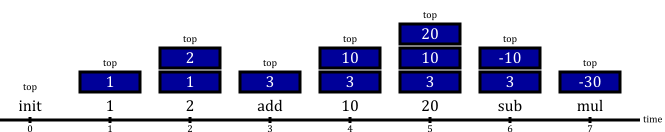
\includegraphics[width=\linewidth]{images/pola.anime.eps}
\caption{\texttt{1 2 + 10 20 - *}.\label{fig:math}}
\end{figure}

以下に、四則演算を行う計算機の実装を示す。\texttt{Stack}型を継承し、\figref{math}に示した手順で、数式の値を逐次的に求める。
式は、空白で区切られた整数と演算子の列である。整数を読み取るとスタックに積み、演算子を読み取ると演算を行う。

\begin{Verbatim}{Scala}
object ArithStackMachine extends collection.mutable.Stack[Int]() {
	def apply(program: String): Int = program.split(" +").map {
		case "+" => push(((a: Int, b: Int) => b + a)(pop(), pop()))
		case "-" => push(((a: Int, b: Int) => b - a)(pop(), pop()))
		case "*" => push(((a: Int, b: Int) => b * a)(pop(), pop()))
		case "/" => push(((a: Int, b: Int) => b / a)(pop(), pop()))
		case num => this.push(num.toInt)
	}.lastOption.map(_ => pop()).last
}
\end{Verbatim}

この実装は、\chapref{math}で再び使用する。\chapref{math}では、中置記法の数式を逆ポーランド記法に変換するコンパイラを実装する。

\begin{Verbatim}{Scala}
println(ArithStackMachine("1 2 + 10 20 - *")) // -30
println(ArithStackMachine("3 4 * 10 20 * +")) // 212
println(ArithStackMachine("5 6 10 + 20 * +")) // 325
println(ArithStackMachine("7 8 10 * 20 - *")) // 420
\end{Verbatim}

\chapter{万能な計算モデル\label{chap:turing}}

\chapref{turing}では、記憶装置を備えた有限状態機械を解説する。再帰計算に対応し、可能な計算の範囲はラムダ計算に匹敵する。

\section{セルオートマトン\label{sect:cell}}

\textbf{セル}と呼ばれる有限状態機械が縦横に並び、各々$k$個の隣接セルの状態を参照して、\eqref{cell}により同時に状態遷移する。
%
\begin{equation}
\label{eq:cell}
\delta: Q^k \to Q.
\end{equation}
%
空間に跨る記憶装置を得た恩恵で、再帰的な情報を表現できる。また、任意の計算機を模倣する遷移規則を設定できる。
例えば、\figref{wire}の\textbf{ワイヤワールド}は、黄色のセルで配線すると、赤青の信号が配線を巡り、様々な論理回路を模倣する。

\begin{figure}[h]
\centering
\subfloat[4bit counter.]{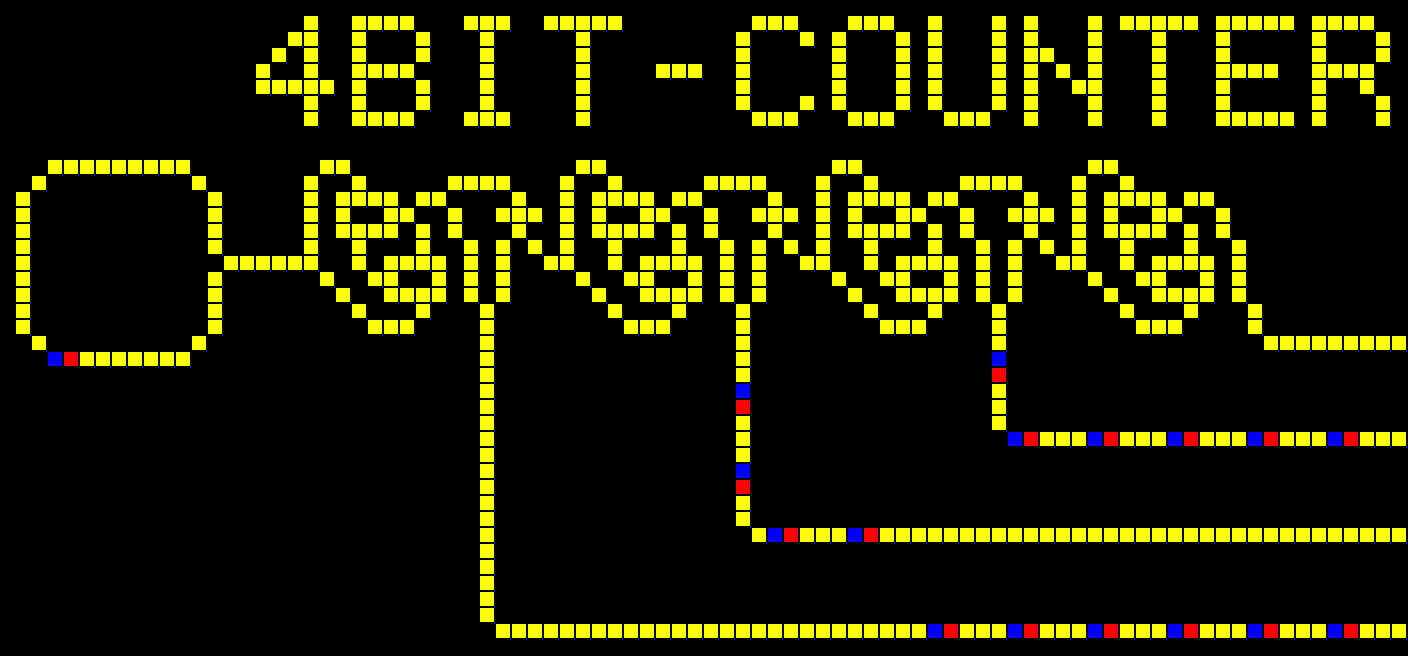
\includegraphics[width=.49\linewidth]{images/wire.count.eps}} \quad
\subfloat[serial adder.]{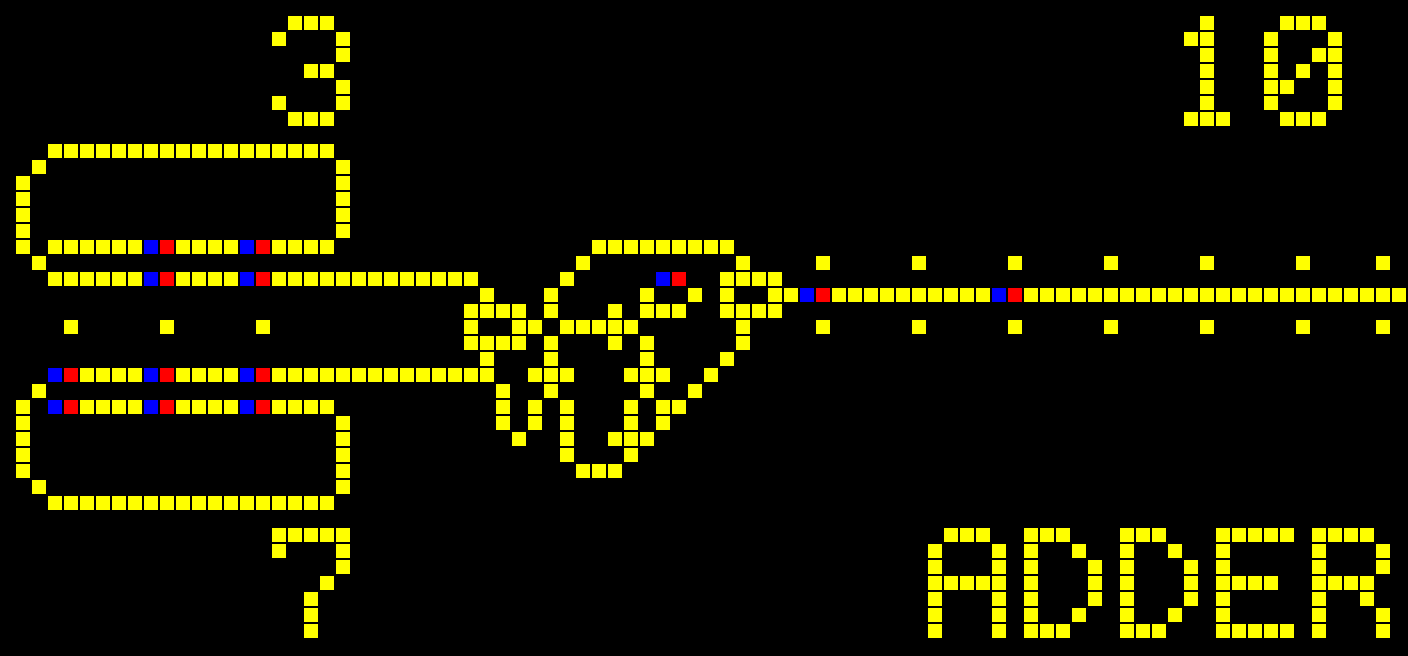
\includegraphics[width=.49\linewidth]{images/wire.adder.eps}}
\caption{wireworld logic circuits.\label{fig:wire}}
\end{figure}

任意の論理回路を自由に配置でき、その様子を言語と捉えれば、\figref{wire}は言語処理系と等価である。以下に実装を示す。

\begin{Verbatim}{Scala}
class CA2[S](rule: Seq[Seq[S]] => S, d: Int = 1) {
	def ROI[V](i: Int)(s: Seq[V]) = Range.inclusive(i - d, i + d).map(Math.floorMod(_, s.size)).map(s)
	def apply(s: Seq[Seq[S]]) = s.indices.map(x => s(x).indices.map(y => rule(ROI(x)(s).map(ROI(y)))))
}
\end{Verbatim}

\texttt{rule}が遷移規則で、\texttt{apply}が状態遷移を表す。\texttt{ROI}が隣接セルである。具体的な遷移規則は、\texttt{CA2}型を継承して定義する。

\begin{Verbatim}{Scala}
object WireWorldRule extends CA2[Char](ROI => ROI(1)(1) match {
	case 'W' if(ROI.flatten.count(_ == 'H') == 1) => 'H'
	case 'W' if(ROI.flatten.count(_ == 'H') == 2) => 'H'
	case 'W' => 'W'
	case 'H' => 'T'
	case 'T' => 'W'
	case 'B' => 'B'
})
\end{Verbatim}

以下は\textbf{ライフゲーム}の定義である。生命の進化や淘汰を思わせる複雑な模様を描き、やはり任意の計算機を模倣できる。

\begin{Verbatim}{Scala}
object LifeGameRule extends CA2[Char](ROI => ROI(1)(1) match {
	case 'L' if(ROI.flatten.count(_ == 'L') == 3) => 'L'
	case 'L' if(ROI.flatten.count(_ == 'L') == 4) => 'L'
	case 'D' if(ROI.flatten.count(_ == 'L') == 3) => 'L'
	case  _  => 'D'
})
\end{Verbatim}

\section{チューリング機械}

\textbf{チューリング機械}は、無限長の\textbf{テープ}と、その内容を読み書きする有限状態機械と、\eqref{tape}の遷移関数$\delta$で構成される。
状態$q_n$で記号$x_n$を読み取ると、記号$y_n$に書き換える。状態$q_{n+1}$に遷移して$\lambda_n$の方向に移動し、再び記号を読み取る。
%
\begin{equation}
\label{eq:tape}
(q_{n+1},y_n,\lambda_n) = \delta(q_n,x_n),
\where
\left\{
\begin{aligned}
q_n &\in Q,\\
x_n,y_n &\in \Sigma,\\
\lambda_n &\in \{L,R\}.
\end{aligned}
\right.
\end{equation}
%
逐次処理型の計算機と理論的に等価であり、実行可能な計算は、並列処理型の万能機械であるセルオートマトンに並ぶ。
特に、\textbf{帰納的に枚挙可能}な集合の計算が得意である。2進数で与えられた自然数の後続を求める手順を、\figref{tape}に示す。

\begin{figure}[h]
\centering
\subfloat[\texttt{100=011+001}.]{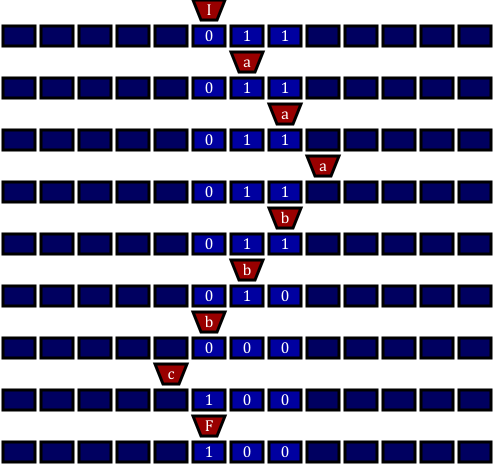
\includegraphics[width=.32\linewidth]{images/tape.plus1.eps}} \quad
\subfloat[\texttt{110=101+001}.]{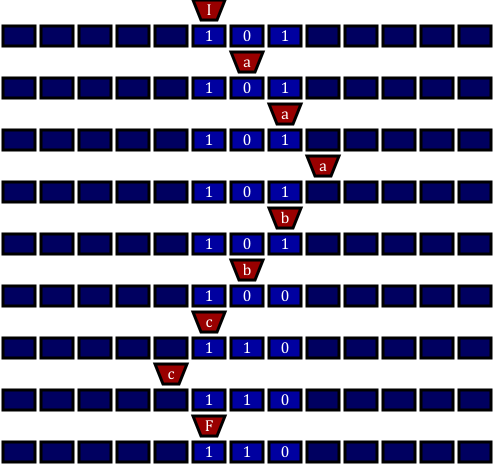
\includegraphics[width=.32\linewidth]{images/tape.plus2.eps}} \quad
\subfloat[\texttt{111=110+001}.]{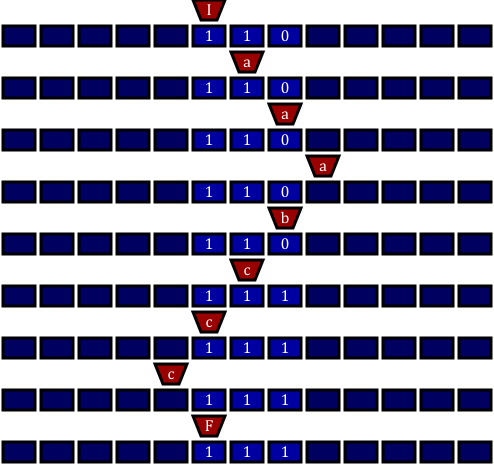
\includegraphics[width=.32\linewidth]{images/tape.plus3.eps}}
\caption{numerical increment operation on a Turing machine ($k=1$).\label{fig:tape}}
\end{figure}

任意の遷移関数を読み取り、その遷移関数を忠実に実行する、言語処理系と等価な\textbf{万能チューリング機械}も実装できる。
遷移関数と計算手順で、異なるテープを使用した例を\texttt{UTM}型に実装する。状態0から1にかけて、遷移規則を検索する。

\begin{Verbatim}{Scala}
class UTM[V](data1: Seq[V], data2: Seq[V], b1: V, b2: V, mL: V, mR: V, var s1: V, var s2: Int = 0) {
	val tape1 = data1.zipWithIndex.map(_.swap).to(collection.mutable.SortedMap)
	val tape2 = data2.zipWithIndex.map(_.swap).to(collection.mutable.SortedMap)
	var hd1 = 0
	var hd2 = 0
	def r1 = tape1.getOrElse(hd1, b1)
	def r2 = tape2.getOrElse(hd2, b2)
	def apply(sop: V) = Iterator.continually(s2 match {
		case 0 if r2 == s1 => (s1 = s1, s2 = 1, tape1(hd1) = r1, hd1 += 0, hd2 += 1)
		case 0 if r2 != s1 => (s1 = s1, s2 = 0, tape1(hd1) = r1, hd1 += 0, hd2 += 5)
		case 1 if r2 == r1 => (s1 = s1, s2 = 2, tape1(hd1) = r1, hd1 += 0, hd2 += 1)
		case 1 if r2 != r1 => (s1 = s1, s2 = 0, tape1(hd1) = r1, hd1 += 0, hd2 += 4)
		case 2 if r2 != b2 => (s1 = r2, s2 = 3, tape1(hd1) = r1, hd1 += 0, hd2 += 1)
		case 3 if r2 != b2 => (s1 = s1, s2 = 4, tape1(hd1) = r2, hd1 += 0, hd2 += 1)
		case 4 if r2 == b1 => (s1 = s1, s2 = 5, tape1(hd1) = r1, hd1 += 0, hd2 += 1)
		case 4 if r2 == mL => (s1 = s1, s2 = 5, tape1(hd1) = r1, hd1 -= 1, hd2 += 1)
		case 4 if r2 == mR => (s1 = s1, s2 = 5, tape1(hd1) = r1, hd1 += 1, hd2 += 1)
		case 5 if r2 == b2 => (s1 = s1, s2 = 0, tape1(hd1) = r1, hd1 += 0, hd2 += 1)
		case 5 if r2 != b2 => (s1 = s1, s2 = 5, tape1(hd1) = r1, hd1 += 0, hd2 -= 1)
	}).takeWhile(t => s1 != sop || s2 != 0).map(t => tape1.values.mkString)
}
\end{Verbatim}

状態2から4にかけて、状態遷移と書き戻しと移動を行う。状態5でテープの左端に戻り、状態0に戻る。使用例を示す。
遷移規則は\eqref{tape}の通り、5個組で読み込ませる。初期状態\texttt{I}から状態\texttt{F}まで動かすと、\figref{tape}の計算が実行される。

\begin{Verbatim}{Scala}
case class CUTM(data1: String, data2: String) extends UTM(data1, data2, ' ', '*', 'L', 'R', 'I')
CUTM("0111111", "I0a0RI1a1Ra0a0Ra1a1Ra b Lb0c1Lb1b0Lb F1 c0c0Lc1c1Lc F R")('F').foreach(println)
\end{Verbatim}

\chapter{型付きラムダ計算\label{chap:lambda}}

実在する計算機を意識した\chapref{automata}の計算モデルに対し、関数の\textbf{評価}と\textbf{適用}による計算手順の抽象化がラムダ計算である。
\chapref{lambda}では、任意の式を\textbf{ラムダ式}と呼ぶ。変数も、整数も、関数もラムダ式である。関数は、\eqref{abs}のように定義する。
%
\begin{equation}
\label{eq:abs}
f \coloneqq \lambda xy.2x+3y+z+1.
\end{equation}
%
\eqref{abs}を関数$f$の\textbf{ラムダ抽象}と呼ぶ。変数$x$と$y$を、$\lambda$により\textbf{束縛}された変数と呼ぶ。また、変数$z$を\textbf{自由変数}と呼ぶ。
\eqref{abs}は\eqref{curry}と等価である。関数$g$は、変数$x$を束縛し、変数$y$を引数に取る関数を返す。これを\textbf{カリー化}と呼ぶ。
%
\begin{equation}
\label{eq:curry}
g \coloneqq \lambda x.\lambda y.2x+3y+z+1.
\end{equation}
%
\eqref{app}は、変数$x$と$y$を具体的な値で束縛する。これを関数適用と呼ぶ。また、式の実体を計算する操作を評価と呼ぶ。
評価の途中で、束縛変数を定数に置換する操作を\textbf{ベータ簡約}と呼ぶ。\eqref{app}の値は、2度の簡約を経由して$27$と求まる。
%
\begin{equation}
\label{eq:app}
\lambda x.\lambda y.(3x+7y) \enspace 2 \enspace 3 \app \lambda y.(6+7y) \enspace 3 \app 6+21 = 27.
\end{equation}

\section{万能性}

任意の自然数と演算は、自然数を枚挙する関数$s$と自然数$0$があれば、\textbf{ペアノの公理}で定義できる。\eqref{num}に例を示す。
自然数は、2個の引数を取る関数で表す。変数$x$に自然数を渡せば、加算になる。変数$s$に自然数を渡せば、乗算になる。
%
\begin{equation}
\label{eq:num}
n \coloneqq \lambda sx.(s^{\circ n}x) \enspace \lambda x.(x+1) \enspace 0,
\enspace
\left\{
\begin{aligned}
a + b &\coloneqq \lambda ab.\lambda sx.as(bsx),\\
a \times b &\coloneqq \lambda ab.\lambda sx.a(bs)x.
\end{aligned}
\right.
\end{equation}
%
真偽値は、真と偽の順序組を引数に取り、どちらかを返す関数で表現できる。論理積と論理和の定義例を\eqref{bool}に示す。
真偽値の変数$y$を偽で束縛すれば、変数$x$との論理積になる。逆に、変数$x$を真で束縛すれば、変数$y$との論理和になる。
%
\begin{equation}
\label{eq:bool}
\mathrm{t} \coloneqq \lambda xy.x, \enspace
\mathrm{f} \coloneqq \lambda xy.y, \enspace
\left\{
\begin{aligned}
a \land b &\coloneqq \lambda ab.ab\mathrm{f},\\
a \lor  b &\coloneqq \lambda ab.a\mathrm{t}b.
\end{aligned}
\right.
\end{equation}
%
再帰計算は、任意の関数$f$の\textbf{不動点}を求める関数$p$が存在し、即ち\eqref{fix}を満たす場合に、無名関数の形で表現できる。
%
\begin{equation}
\label{eq:fix}
\forall f, \enspace f(p(f)) \equiv p(f).
\end{equation}
%
例えば、関数$g$を任意の再帰計算とし、\eqref{rec}に示す関数$h$を定義すると、関数$g$は関数$h$と変数$x$を引数に受け取る。
%
\begin{equation}
\label{eq:rec}
h \coloneqq \lambda x.pgx
\equiv \lambda x.(pg)x
\equiv \lambda x.(g (pg)) x
\equiv \lambda x.ghx
, \where g \coloneqq \lambda fy.E.
\end{equation}
%
関数$h$を通じて、関数$g$が再帰的に参照される。任意の関数の不動点を与える関数$p$の、最も著名な例を\eqref{Y}に示す。
%
\begin{equation}
\label{eq:Y}
\Yc{} \coloneqq \lambda f.(\lambda x.f(xx))(\lambda x.f(xx)).
\end{equation}
%
関数$f$に対し、\eqref{Y}の関数$\Yc$が\eqref{fix}を満たす様子は、\eqref{Yf}で証明できる。ただし、無限再帰に注意を要する。
例えば、式$\Yc{}fx$を評価すると、無限に\eqref{Yf}が展開される。対策として、\chapref{fava}で解説する非正格評価が必要になる。
%
\begin{equation}
\label{eq:Yf}
\Yc{}f
\app (\lambda x.f(xx))(\lambda x.f(xx))
\app f((\lambda x.f(xx))(\lambda x.f(xx)))
\equiv f(\Yc{}f).
\end{equation}
%
関数$\Yc$と等価な関数$\Zc$を利用する方法もある。\eqref{Z}に示す関数$\Zc{}$は、関数$\Yc$に\textbf{イータ変換}の逆を施した関数である。
%
\begin{equation}
\label{eq:Z}
\Zc{} \coloneqq \lambda f.(\lambda x.f(\lambda y.xxy))(\lambda x.f(\lambda y.xxy)).
\end{equation}
%
\eqref{Zf}を評価すると、右辺の関数が出現し、実際に引数$y$を渡すまで\eqref{Zf}の展開が保留され、無限再帰を防げる。
%
\begin{equation}
\label{eq:Zf}
\Zc{}f
\app (\lambda x.f(\lambda y.xxy))(\lambda x.f(\lambda y.xxy))
\app f(\lambda y.(\lambda x.f(\lambda y.xxy))(\lambda x.f(\lambda y.xxy))y)
\app f(\lambda y.\Zc{}fy).
\end{equation}
%
以上で、算術や論理計算や再帰計算を含む、理論的な裏付けが揃った。\chapref{favac}で言語処理系が完成したら、実験しよう。

\section{型推論}

\textbf{型付きラムダ計算}は、命題論理の規則に従って、式の型を推論し、型の矛盾や無限再帰を形式的に検出する体系である。
簡単に命題論理を復習する。命題$P$が命題$Q$を、命題$Q$が命題$R$を含意する場合に、\eqref{infer}の\textbf{三段論法}が成立する。
%
\begin{equation}
\label{eq:infer}
\infer{P \to R}{P \to Q & Q \to R}.
\end{equation}
%
命題論理では、命題の妥当性は、演繹の累積で証明される。この過程は、命題の集合$\Gamma$を仮定して、\eqref{proof}で表せる。
%
\begin{equation}
\label{eq:proof}
\Gamma \vdash P \to R,
\where
\left\{
\begin{aligned}
P \to Q \in \Gamma, \\
Q \to R \in \Gamma.
\end{aligned}
\right.
\end{equation}
%
型付きラムダ計算では、集合$\Gamma$を\textbf{型環境}と呼ぶ。具体的には、変数や部分式に設定した型の情報を格納した配列である。
曖昧な型は変数で表す。例えば、自由変数$x$の型は未知なので、変数$\sigma$が環境$\Gamma$に格納され、式$x$の型は$\sigma$と推論される。
%
\begin{equation}
\infer{\Env{x: \sigma}}{\Gamma(x) \coloneqq \sigma}.
\end{equation}
%
関数$f$の型を推論しよう。過程を\eqref{type:fun}に示す。関数は、含意の記号$\to$を利用して、定義域と値域の組で表現できる。
%
\begin{equation}
\label{eq:type:fun}
\infer{\Env{f: \sigma \to \tau}}{x: \sigma \vdash E: \tau & f \coloneqq \lambda x. E}
\end{equation}
%
\eqref{type:fun}を含意$\to$の\textbf{導入規則}と呼ぶ。最後に、関数$f$の適用$fx$の型を推論する。\eqref{type:app}を含意$\to$の\textbf{除去規則}と呼ぶ。
%
\begin{equation}
\label{eq:type:app}
\infer{\Env{f x: \tau}}{\Env{f: \sigma \to \tau} & \Env{x: \sigma}}
\end{equation}
%
型推論の過程では、型変数が満たす制約条件の組が生成され、その全てを満たす型が解となる。\eqref{type:ex}の例で考える。
%
\begin{equation}
\label{eq:type:ex}
(\lambda x.xy)(zy).
\end{equation}
%
推論の過程を\eqref{type:ex:var}に示す。同じ変数には、同じ型変数を設定する。推論の過程で、型変数の制約条件が生成される。
%
\begin{equation}
\label{eq:type:ex:var}
\infer{
(\lambda x.xy)(zy): \sigma
\mid \alpha \to \mu = \nu \to \sigma
\mid \alpha = \beta \to \mu
\mid \gamma = \beta \to \nu
}{
\infer{
\lambda x.xy: \alpha \to \mu \mid \alpha = \beta \to \mu
}{
\infer{xy: \mu \mid \alpha = \beta \to \mu}{x: \alpha & y: \beta}
}
&
\infer{zy: \nu \mid \gamma = \beta \to \nu}{z: \gamma & y: \beta}
}
\end{equation}
%
代数学の要領で制約条件を消去し、解を得る作業を\textbf{単一化}と呼ぶ。特に、関数の型を分解する。\eqref{type:ex:infer}に過程を示す。
%
\begin{equation}
\label{eq:type:ex:infer}
\infer{
\gamma = \beta \to \beta \to \sigma
}{
\infer{\alpha = \beta \to \sigma}{\infer{\mu = \sigma}{\alpha \to \mu = \nu \to \sigma} & \alpha = \beta \to \mu}
&
\infer{\gamma = \beta \to \alpha}{\infer{\alpha = \nu}{\alpha \to \mu = \nu \to \sigma} & \gamma = \beta \to \nu}
}
\end{equation}
%
\eqref{type:ex:infer}の例では、全ての制約条件を消去できた。それでも、型変数$\beta,\sigma$は任意の型になり得る。これを\textbf{多相型}と呼ぶ。
なお、再帰関数の型推論では、\eqref{type:rec}に示す\textbf{同値再帰型}が出現する。無闇に\eqref{type:rec}を展開すると、無限再帰に陥る。
%
\begin{equation}
\label{eq:type:rec}
\sigma = \sigma \to \tau.
\end{equation}
%
\eqref{Yf}を例に考える。\eqref{type:Y}に示す推論により、型$\phi,\psi$は再帰型と判明する。その時点で推論を終える必要がある。
%
\begin{equation}
\label{eq:type:Y}
\infer{
(\lambda x.f(xx))(\lambda x.f(xx)): \sigma
\mid \phi \to \rho = (\psi \to \tau) \to \sigma
\mid \eta = \mu \to \rho \mid \phi = \phi \to \mu
\mid \eta = \nu \to \tau \mid \psi = \psi \to \nu
}{
\infer{
\lambda x.f(xx): \phi \to \rho
\mid \eta = \mu \to \rho \mid \phi = \phi \to \mu
}{
\infer{
f(xx): \rho
\mid \eta = \mu \to \rho \mid \phi = \phi \to \mu
}{
\infer{xx: \mu \mid \phi = \phi \to \mu}{x: \phi} & f: \eta
}
}
&
\infer{
\lambda x.f(xx): \psi \to \tau
\mid \eta = \nu \to \tau \mid \psi = \psi \to \nu
}{
\infer{
f(xx): \tau
\mid \eta = \nu \to \tau \mid \psi = \psi \to \nu
}{
\infer{xx: \nu \mid \psi = \psi \to \nu}{x: \psi} & f: \eta
}
}
}
\end{equation}
%
同値再帰型を表す特殊な型変数を実装すれば、再帰関数の型推論も可能だが、誤った式に意図せず型が付く場合もある。

\chapter{簡単なコンパイラ\label{chap:math}}

\chapref{automata}の計算モデルは、C言語やラムダ計算など\textbf{高水準言語}の内容を実行するには原始的すぎる。そこで、翻訳を行う。
翻訳を行う言語処理系を\textbf{コンパイラ}と呼ぶ。\chapref{math}では、簡単な逆ポーランド記法の翻訳を例に、その概念を解説する。

\section{形式言語の階層性\label{sect:lang}}

\textbf{形式言語}とは、定義が明確で、何らかの計算手順で処理できる言語である。まず、形式言語$L$は\eqref{lang}で定義される。
%
\begin{equation}
\label{eq:lang}
L(G) \subset \Sigma^* = \left\{\langle\sigma_1,...,\sigma_n,...\rangle\mid\sigma_n\in\Sigma\right\}.
\end{equation}
%
言語$L$は\textbf{文}の集合である。文とは、記号$\sigma$の列である。記号は有限集合$\Sigma$で定義され、集合$\Sigma$を\textbf{アルファベット}と呼ぶ。
記号$\sigma$の出現には、明確な規則がある。この規則を\textbf{生成規則}と呼び、生成規則の集合を\textbf{文法}と呼ぶ。\eqref{gen}に例を示す。
%
\begin{equation}
\label{eq:gen}
P = \left\{
\begin{aligned}
\mathtt{S} &\to \texttt{(S)},\\
\mathtt{S} &\to \texttt{(f)},
\end{aligned}
\right.:(N\cup\Sigma)^*\to(N\cup\Sigma)^*.
\end{equation}
%
生成規則は、左辺の記号列を右辺の記号列に置換する規則である。\eqref{gen}の例では、記号\texttt{S}から\eqref{fs}が導出される。
%
\begin{equation}
\label{eq:fs}
\texttt{(f)},
\texttt{((f))},
\texttt{(((f)))},
\texttt{((((f))))},
\texttt{(((((f)))))},
\texttt{((((((f))))))},
\texttt{(((((((f)))))))},
\texttt{((((((((f))))))))},
\ldots.
\end{equation}
%
生成規則の両辺に出現できる記号$\nu\!\in\!N$を\textbf{非終端記号}と呼ぶ。また、右辺に限って出現する記号$\sigma\!\in\!\Sigma$を\textbf{終端記号}と呼ぶ。
任意の文は、\textbf{開始記号}と呼ばれる記号$S$を起点に生成される。最終的に、言語$L(G)$の文法$G$は\eqref{gram}で定義される。
%
\begin{equation}
\label{eq:gram}
G=(N,\Sigma,P,S),\where S\in N.
\end{equation}
%
文法$G$に従う文を生成し、または文を開始記号$S$に帰する手順が定義され、曖昧性がなければ、文法$G$は\textbf{形式的}である。
形式言語の中でも、生成規則が自由な言語を\textbf{帰納的可算言語}と呼び、\eqref{csg}の制限を加えた言語を\textbf{文脈依存言語}と呼ぶ。
%
\begin{equation}
\label{eq:csg}
\alpha A \beta \to \alpha \gamma \beta,
\where
\left\{
\begin{aligned}
A &\in N,\\
\alpha,\beta &\in (N\cup\Sigma)^*,\\
\gamma &\in (N\cup\Sigma)^+.
\end{aligned}
\right.
\end{equation}
%
形式言語の中でも、\eqref{cfg}の制限を持ち、前後の文脈に依存せずに、生成規則が適用できる言語を\textbf{文脈自由言語}と呼ぶ。
\sectref{pola}で述べたプッシュダウンオートマトンを利用して、文に対して生成規則を再帰的に適用することで処理できる。
%
\begin{equation}
\label{eq:cfg}
A \to \alpha,
\where
\left\{
\begin{aligned}
A &\in N,\\
\alpha &\in (N\cup\Sigma)^*.
\end{aligned}
\right.
\end{equation}
%
形式言語の中でも、文法の制約が強く、有限状態機械で処理可能な言語を\textbf{正規言語}と呼ぶ。その記法が正規表現である。
有限状態機械では、無限の記憶を持てず、特に再帰的な生成規則を扱えず、生成規則は\eqref{reg}に示す形式に制限される。
%
\begin{equation}
\label{eq:reg}
\left\{
\begin{aligned}
A &\to a,\\
A &\to aB,
\end{aligned}
\right.
\where
\left\{
\begin{aligned}
a &\in \Sigma,\\
A,B &\in N.
\end{aligned}
\right.
\end{equation}
%
形式言語の文は、適用した生成規則の木構造で表現できる。これを\textbf{構文木}と呼び、構文木を導く作業を\textbf{構文解析}と呼ぶ。
特にLL法では、終端記号の列を読み進め、見つけた終端記号に適う生成規則を、開始記号$S$を起点に深さ優先探索する。
%
\begin{equation}
(S=\texttt{add})\to(\texttt{mul + mul})\to(\texttt{num * num + num})\to(\texttt{1 * 2 + 3}).
\end{equation}
%
LR法では、終端記号の列を読み進め、置換可能な部分を非終端記号に置換する。最終的に開始記号$S$に到達して終わる。
%
\begin{equation}
(\texttt{1 * 2 + 3})\to(\texttt{num * num + num})\to(\texttt{mul + mul})\to(S=\texttt{add}).
\end{equation}
%
通常、高水準言語は形式言語である。仮に自然言語を採用すると、翻訳する手順が曖昧になり、実装困難なためである。

\section{解析表現文法の例\label{sect:PEG}}

形式文法は、構文解析の際には曖昧になる。そこで、生成規則ではなく、構文解析の手順を形式的に定義した文法もある。
\textbf{解析表現文法}はその例である。解析表現文法は、文脈依存言語の部分集合を扱う。簡単な四則演算を定義する例を示す。

\begin{table}[h!]
\raggedright
\begin{tabular}{@{}Bl}
加減算 & \verb#add ::= mul (('+' / '-') mul)*# \\
乗除算 & \verb#mul ::= num (('*' / '/') num)*# \\
整数値 & \verb#num ::= [0-9]+ / '(' add ')'#
\end{tabular}
\end{table}

左辺が非終端記号で、右辺が非終端記号と終端記号の列を表す。ただし、右辺に出現する記号には、以下の意味がある。

\begin{table}[h!]
\raggedright
\begin{tabular}{@{}ll}
\verb# *# & 直前の記号が0回以上出現する。\\
\verb# +# & 直前の記号が1回以上出現する。\\
\verb# ?# & 直前の記号が出現する場合がある。\\
\verb# /# & 直前または直後の記号が出現する。\\
\verb#()# & 括弧内の記号列をひと纏めにする。\\
\verb#''# & 引用内の字句がそのまま出現する。\\
\verb#[]# & 範囲内の記号が選択的に出現する。\\
\verb# &# & 直後の記号が出現すれば成功する。\\
\verb# !# & 直後の記号が出現すれば失敗する。\\
\end{tabular}
\end{table}

解析表現文法はLL法の亜種である\textbf{再帰下降構文解析}を定義する記法である。これは、再帰的な関数で構文解析器を表す。
様々な言語を定義可能だが、非終端記号を置換すると再び左に出現する\textbf{左再帰}の言語では、無限再帰に陥る欠点がある。

\begin{table}[h]
\raggedright
\begin{tabular}{@{}Bl}
左再帰 & \verb#add ::= add ('+' / '-') mul / mul#
\end{tabular}
\end{table}

左再帰は、\textbf{左結合}の式を表す際に重要である。\eqref{left}に例を示す。左結合の式では、式の左側の演算子が優先される。
%
\begin{equation}
\label{eq:left}
1 - 2 - 3 - 4 - 5 = (((1 - 2) - 3) - 4) - 5 = -13.
\end{equation}
%
右結合にすれば無限再帰を回避できるが、式の意味が変化してしまう。反復を表す特殊記号\texttt{*}など、代替手段で回避する。

\section{構文解析器の実装\label{sect:parsec}}

\sectref{parsec}では、\sectref{regex}で解説した正規表現の処理系を改良して、解析表現文法に基づく\textbf{パーサコンビネータ}を実装する。
以下の\texttt{PEG}型を継承した\textbf{高階関数}を組み合わせ、再帰下降構文解析器を構築する。構文解析に成功すると、結果を返す。

\begin{Verbatim}{Scala}
class PEG[+M](f: String => Option[Out[M]]) {
	def skip = Reg("""\s*""".r) ~> this <~ Reg("""\s*""".r)
	def / [R >: M](q: => PEG[R]): PEG[R] = new Alt(this, q)
	def ~ [R](q: => PEG[R]): PEG[(M, R)] = new Cat(this, q)
	def <~[R](q: => PEG[R]) = this ~ q ^ (_._1)
	def ~>[R](q: => PEG[R]) = this ~ q ^ (_._2)
	def ^ [T](f: M => T) = new Map(this, f)
	def * = new Rep(this)
	def ? = new Opt(this)
	def apply(in: String) = f(in)
}
\end{Verbatim}

構文解析器は、その構文解析器で構築した構文木と、構文解析器が読み残した終端記号の列を返す。\texttt{Out}型に実装する。

\begin{Verbatim}{Scala}
case class Out[+M](m: M, in: String) {
	def tuple[R](o: Out[R]) = Out(m -> o.m, o.in)
	def apply[R](p: PEG[R]) = p(in).map(tuple(_))
	def toSome = Out(Some(m), in)
}
\end{Verbatim}

最初に、最も単純な構文解析器を実装する。\texttt{Str}型は、指定された終端記号列を左端に発見すると、その記号列を返す。
\texttt{Reg}型は、正規表現で指定された終端記号列を左端に発見すると、その記号列を返す。両者を総称して\textbf{字句解析器}と呼ぶ。

\begin{Verbatim}{Scala}
case class Str(p: String) extends PEG(s => Option.when(s.startsWith(p))(Out(p, s.substring(p.length))))
case class Reg(p: Regex) extends PEG(p.findPrefixMatchOf(_).map(m => Out(m.matched, m.after.toString)))
\end{Verbatim}

\texttt{Alt}型は、1個目の構文解析器が構文解析に成功すると、その結果を返し、失敗した場合は、2個目の構文解析器を試す。
\texttt{Cat}型は、1個目の構文解析器を試してから、読み残した終端記号列に2個目の構文解析器を試し、結果を結合して返す。

\begin{Verbatim}{Scala}
class Alt[L, R >: L](p: => PEG[L], q: => PEG[R]) extends PEG[R](s => p(s) orElse q(s))
class Cat[+L, +R](p: => PEG[L], q: => PEG[R]) extends PEG(p(_).map(_ apply q).flatten)
\end{Verbatim}

\texttt{Map}型は、指定された構文解析器を試し、その結果に対して、関数を適用する。構文木に何らかの加工を施す際に使う。
\texttt{Opt}型は、省略可能な構文を表す。指定された構文解析器を試すが、構文解析に失敗した場合でも、成功したと見做す。

\begin{Verbatim}{Scala}
class Map[+S, +T](p: => PEG[S], f: S => T) extends PEG[T](p(_).map(t => Out(f(t.m), t.in)))
class Opt[+T](p: => PEG[T]) extends PEG(s => p(s).map(_.toSome).orElse(Some(Out(None, s))))
\end{Verbatim}

\texttt{And}型と\texttt{Not}型は、先読みを行う。指定された構文解析器を試すが、読み取り位置を進めず、構文解析の成否のみを返す。
LL法でも先読み可能だが、正規表現で切り出した字句の先読みに限定されるため、解析表現文法よりも表現能力が劣る。

\begin{Verbatim}{Scala}
class And[+T](p: => PEG[T]) extends PEG(s => if(p(s).isDefined) Some(Out(None, s)) else None)
class Not[+T](p: => PEG[T]) extends PEG(s => if(p(s).isDefined) None else Some(Out(None, s)))
\end{Verbatim}

\texttt{Rep}型は、記号の反復を表す。読み取り位置を進めては構文解析を実行し、構文解析に失敗すると、結果を結合して返す。

\begin{Verbatim}{Scala}
class Rep[+T](p: => PEG[T]) extends PEG(s => {
	def ca(a: Out[T]): Out[Seq[T]] = Out(a.m +: re(a.in).m, re(a.in).in)
	def re(s: String): Out[Seq[T]] = p(s).map(ca).getOrElse(Out(Nil, s))
	Some(re(s))
})
\end{Verbatim}

次に、特殊な構文解析器を実装する。\texttt{Fold}型は、左結合する中置記法の式を表す。無限再帰を回避する代替手段である。
1個目の構文解析器は、被演算子を表す。2個目の構文解析器は演算子を表し、演算子の左右に並ぶ被演算子を結合する。

\begin{Verbatim}{Scala}
class Fold[T](p: => PEG[T], q: => PEG[(T, T) => T]) extends PEG({
	(p ~ (q ~ p).*)^(x => x._2.foldLeft(x._1)((l, r) => r._1(l, r._2)))
} apply(_))
\end{Verbatim}

最後に実装する\texttt{Sep}型は、\texttt{Rep}型の特殊な場合で、区切り文字で区切られた記号の反復を表す。区切り文字は廃棄される。

\begin{Verbatim}{Scala}
class Sep[T](p: => PEG[T], q: => PEG[_]) extends Fold[Seq[T]](p.? ^ (_.toSeq), q^(_ => _ ++ _))
\end{Verbatim}

最終的な構文解析器を、以下の\texttt{PEGs}型を継承して実装すると、文字列や正規表現は、暗黙的に構文解析器に変換される。

\begin{Verbatim}{Scala}
class PEGs {
	implicit def implicitText(p: String): PEG[String] = new Str(p).skip
	implicit def implicitRegex(p: Regex): PEG[String] = new Reg(p).skip
}
\end{Verbatim}

使用例を示す。この実装は、数式を読み取る機能に加え、逆ポーランド記法の命令列を生成する\textbf{コード生成器}も兼ねる。

\begin{Verbatim}{Scala}
object ArithPEGs extends PEGs {
	def add: PEG[String] = new Fold(mul, ("+" / "-").^(op => (a, b) => s"$a $b $op"))
	def mul: PEG[String] = new Fold(num, ("*" / "/").^(op => (a, b) => s"$a $b $op"))
	def num: PEG[String] = "[0-9]+".r / ("(" ~> add <~ ")")
	def apply(e: String) = +ArithStackMachine(add(e).get.m)
}
\end{Verbatim}

\section{簡単な言語処理系}

\sectref{parsec}の構文解析器でLISPを実装しよう。LISPは、簡素な文法ながら拡張性が高く、実用的な動的型付け言語である。
LISPの式をS式と呼ぶ。変数の名前や数値を表す\textbf{アトム}と、構文木を形成する\textbf{リスト}で構成される。文法も簡潔である。

\begin{Verbatim}{Scala}
object LispPEGs extends PEGs {
	def sexp: PEG[S] = list / quot / real / name
	def list = "(" ~> (sexp.* ^ List) <~ ")"
	def real = "[0-9]+".r ^ (real => Real(BigDecimal(real)))
	def name = """[^'`,@\(\)\s]+""".r ^ (name => Name(name))
	def quot = "'" ~> sexp ^ (Seq(Name("quote"), _)) ^ List
}
\end{Verbatim}

S式の実装を以下に示す。引数の\texttt{exp}は式の文字列である。\texttt{eval}は評価器で、後述する環境を参照して、式の値を返す。

\begin{Verbatim}{Scala}
abstract class S(val exp: String, eval: S => Env => S) {
	override def toString = exp
	def apply(env: Env): S = eval(this)(env)
	def apply(env: Env)(args: Seq[S]): S = apply(env).asInstanceOf[Form].app(args, env)
}
\end{Verbatim}

次にアトムを実装する。変数を表す\texttt{Name}型と、実数値の\texttt{Real}型を以下に示す。他にも論理型や文字列型を実装しよう。

\begin{Verbatim}{Scala}
case class Name(name: String) extends S(name, v => env => env.apply(v))
case class Real(real: BigDecimal) extends S(real.toString, v => _ => v)
\end{Verbatim}

次にリストを実装する。LISPのリストは関数適用として評価される。最初の要素が関数で、残りが引数のリストとなる。

\begin{Verbatim}{Scala}
case class List(list: Seq[S]) extends S(list.mkString("(", " ", ")"), _ => list.head(_)(list.tail))
\end{Verbatim}

次に演算子を実装する。\texttt{Form}型を継承して、関数の定義を表す\texttt{Lambda}型と、\textbf{マクロ}の定義を表す\texttt{Syntax}型を実装する。
関数の場合は、まず引数を評価して、引数を記憶した環境を生成し、最後に関数の値を評価する。これを\textbf{正格評価}と呼ぶ。

\begin{Verbatim}{Scala}
class Form(exp: String, val app: (Seq[S], Env) => S) extends S(exp, v => _ => v)
class Lambda(p: List, v: S, e: Env) extends Form(s"(lambda $p $v)", (a, s) => v(Env(Some(e), p, s(a))))
class Syntax(p: List, v: S, e: Env) extends Form(s"(syntax $p $v)", (a, s) => v(Env(Some(e), p, a))(s))
\end{Verbatim}

対照的にマクロの場合は、引数を評価せず、式のままマクロの内部に展開し、そのマクロを通常の式と同様に評価する。
例えば、C言語の制御構文に相当するマクロも定義できる。次に、環境を実装する。環境は変数の名前と値を記憶する。

\begin{Verbatim}{Scala}
case class Env(out: Option[Env], params: List, args: Seq[S]) {
	val map = params.list.zip(args).to(collection.mutable.Map)
	def apply(name: S): S = {
		if(map.isDefinedAt(name)) map(name)
		else if(out.nonEmpty) out.get(name)
		else sys.error(s"$name undeclared")
	}
	def apply(args: Seq[S]): Seq[S] = args.map(_.apply(this))
}
\end{Verbatim}

最後に、お好みで\texttt{Form}型を継承し、組込み関数や構文を充実させよう。関数とマクロを定義する構文の例を以下に示す。

\begin{Verbatim}{Scala}
object LambdaForm extends Form("lambda", (a, s) => new Lambda(a.head.asInstanceOf[List], a(1), s))
object SyntaxForm extends Form("syntax", (a, s) => new Syntax(a.head.asInstanceOf[List], a(1), s))
\end{Verbatim}

以上で、簡素ながら優れた拡張性と実用性を備えるLISPが完成した。階乗を\texttt{defun}マクロで定義する例を以下に示す。

\begin{Verbatim}{sample}
lisp$ (defun fact (x) (if (eq x 1) x (* x (fact (- x 1)))))
(lambda (x) (if (eq x 1) x (* x (fact (- x 1)))))
\end{Verbatim}

\chapter{自作言語の仕様書\label{chap:fava}}

\fava{}は静的型付け言語である。組込み型には、整数型と実数型と論理型と文字列型と関数型があり、型推論が行われる。
整数型は符号付き32~bit整数で、実数型はIEEE~754~(64~bit~2進数)浮動小数点数で、文字列はUTF-16で表現される。

\begin{table}[h]
\raggedright
\begin{tabular}{@{}Bl}
整数型 & \verb#int  ::= [0-9]+# \\
実数型 & \verb#real ::= [0-9]* ([0-9] '.' / '.' [0-9]) [0-9]*# \\
論理型 & \verb#bool ::= 'true' / 'false'# \\
文字列 & \verb#text ::= '"' [^"]* '"'# \\
関数型 & \verb#func ::= '(' (id (',' id)*)? ')' '=>' expr#
\end{tabular}
\end{table}

識別子は、その識別子が記述された箇所を包含し、識別子と同じ名前の引数を持つ、最も内側の関数の引数を参照する。
関数の内外で変数を宣言または代入する機能はなく、従って、識別子が参照する実体は何らかの関数の引数に限られる。

\begin{table}[h]
\raggedright
\begin{tabular}{@{}Bl}
識別子 & \verb#id ::= [@A-Z_a-z] [@0-9A-Z_a-z]*#
\end{tabular}
\end{table}

引数の値は変更できず、従って識別子を含む式が参照する実体は、状態によらず自明である。これを\textbf{参照透明性}と呼ぶ。
複数の文を逐次的に実行する\textbf{ブロック構文}はなく、関数宣言の構文も省略した。以下に解析表現文法による定義を示す。

\begin{table}[h]
\raggedright
\begin{tabular}{@{}Bl}
ラムダ式 & \verb#expr ::= cond / or# \\
条件分岐 & \verb#cond ::= or  '?' expr ':' expr# \\
論理積   & \verb#or   ::= or  '|' and / and# \\
論理和   & \verb#and  ::= and '&' eql / eql# \\
等値比較 & \verb#eql  ::= eql ('==' / '!=') rel / rel# \\
順序比較 & \verb#rel  ::= rel ('<' / '>' / '<=' / '>=') add / add# \\
加減算   & \verb#add  ::= add ('+' / '-') mul / mul#\\
乗除算   & \verb#mul  ::= mul ('*' / '/' / '%') unr / unr# \\
単項演算 & \verb#unr  ::= ('+' / '-' / '!') unr / call# \\
関数適用 & \verb#call ::= call '(' expr (',' expr) ')' / fact# \\
式の要素 & \verb#fact ::= func / bool / text / real / int / id / '(' expr ')'# \\
\end{tabular}
\end{table}

この定義は左再帰を含む。中置記法の論理演算と比較演算と算術演算は、全て左結合である。単項演算は右結合である。
関数は、他の関数を引数や返り値にできる。これを\textbf{高階関数}と呼ぶ。ただし、関数は宣言できず、従って\textbf{無名関数}である。

\begin{Verbatim}{sample}
fava$ ((function)=>function())(()=>1+2)
3
\end{Verbatim}

高階関数の内部で定義された関数からは、外側の高階関数で定義された引数を参照できる。この関数を\textbf{関数閉包}と呼ぶ。
関数の引数は、その引数を参照する関数閉包が存在し、参照される限り、関数適用が完了しても生存し、参照可能である。

\begin{Verbatim}{sample}
fava$ ((x)=>((y)=>x*y))(2)(3)
6
\end{Verbatim}

引数の値は、関数を呼び出す時点では計算されず、値が必要になった時点で計算される。この動作を\textbf{非正格評価}と呼ぶ。
\textbf{遅延評価}とも呼ばれる。詳細は\chapref{lambda}に述べるが、端的に言えば、再帰的な関数が無限再帰に陥るのを防ぐ効果がある。

\begin{Verbatim}{sample}
fava$ ((f)=>((x)=>f(x(x)))((x)=>f(x(x))))((f)=>(n)=>(n==0)?1:n*f(n-1))(10)
3628800
\end{Verbatim}

\chapter{命令セットを作る\label{chap:VM}}

\chapref{VM}では、\sectref{pola}で実装した計算機を拡張し、\textbf{分岐命令}を備えた\textbf{命令セット}を設計して、条件分岐や関数を実現する。
以下に例を示す。まず、\texttt{Push}命令がスタックに値を積む。その値が偽なら、続く\texttt{Skin}命令が、3個の命令を読み飛ばす。

\begin{Verbatim}{sample}
fava$ compile(true? 12: 34)
Push(true) Skin(3) Push(12) Skip(2) Push(34)
\end{Verbatim}

\texttt{Skip}命令は\textbf{無条件分岐命令}で、条件式の値に依らず指定された個数の命令を読み飛ばす。この例の計算結果は12である。
関数も同様の仕組みで実現できる。関数は、\texttt{Def}命令に始まり、\texttt{Ret}命令に終わる命令列に翻訳される。以下に例を示す。

\begin{Verbatim}{sample}
fava$ compile((x,y)=>0+x+y)
Def(7) Push(0) Load(0,0) IAdd Load(0,1) IAdd Ret
\end{Verbatim}

\texttt{Def}命令は、それに続く命令列を実行する関数をスタックに積む。また、その命令列を読み飛ばし、意図せぬ実行を防ぐ。
\texttt{Ret}命令は、関数の引数を格納した\textbf{環境}を廃棄して、関数を呼び出した位置に復帰する。関数適用の命令列も以下に示す。

\begin{Verbatim}{sample}
fava$ compile(((f)=>f())(()=>3))
Def(4) Load(0,0) Call(0) Ret Def(3) Push(3) Ret Call(1)
\end{Verbatim}

\texttt{Call}命令は、引数と関数をスタックから取り出す。復帰位置を記録して、環境を構築してから、関数の冒頭に移動する。
\figref{call}に動作を示す。上下に2個のスタックがあるが、上のスタックで計算を行う。下のスタックは、環境を格納する。

\begin{figure}[h]
\centering
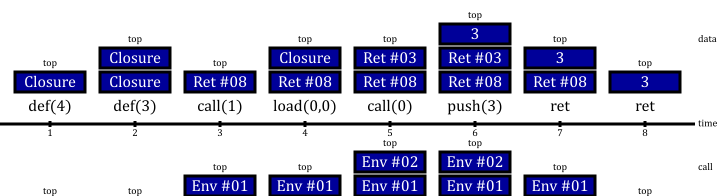
\includegraphics[width=\linewidth]{images/fava.call2.eps}
\caption{function call mechanism for \texttt{((f)=>f())(()=>3)}.\label{fig:call}}
\end{figure}

以上は、引数の値を関数適用の前に求める\textbf{正格評価}の説明である。非正格評価では、引数の値を計算せずに関数を呼ぶ。
条件分岐を含む関数では、引数の値が使用されず廃棄される場合がある。非正格評価であれば、この無駄を解消できる。

\begin{Verbatim}{sample}
fava$ ((x,y,z)=>(x?y:z))(true,3+3,3*3)
6
\end{Verbatim}

引数を無名関数で包み、引数を参照する際にその関数を呼べば、非正格評価と同じ挙動になる。これを\textbf{名前呼び}と呼ぶ。

\begin{Verbatim}{sample}
fava$ ((x,y)=>x()*x()+y())(()=>3+3,()=>3*3)
45
\end{Verbatim}

同じ引数を何度も参照する場合は、値を再利用すると効率的である。これを\textbf{必要呼び}と呼ぶ。詳細は\sectref{lazy}に述べる。

\begin{Verbatim}{sample}
fava$ compile(((x)=>x)(5))
Def(11) Load(0,0) Nil Skin(6) Ref Call(0) Load(0,0) Fix Set Get Ret Def(3) Push(5) Ret Arg Call(1)
\end{Verbatim}

\section{命令の基本設計}

命令は、\texttt{Code}型を継承する。\texttt{FaVM}型は、実行環境の本体である。命令は、所定の操作を実行し、変数\texttt{pc}を繰り上げる。

\begin{Verbatim}{Scala}
class Code(op: FaVM => Unit) {
	def apply(vm: FaVM) = (op(vm), vm.pc += 1)
}
\end{Verbatim}

変数\texttt{pc}は、\textbf{プログラムカウンタ}に相当する。これは、命令を実行する度に繰り上がり、次に実行する命令の位置を示す。

\section{関数の基本設計\label{sect:func}}

次に、関数の仕組みを実装する。関数は、関数が実行する最初の命令の位置と、関数を生成した時点の環境を参照する。
関数が参照する環境は、この関数を包み込む関数の引数を格納した環境である。関数閉包を実現するための布石である。

\begin{Verbatim}{Scala}
case class Closure(from: Int, out: Env)
\end{Verbatim}

遅延評価の仕組みも実装する。遅延評価は、関数の引数を包む関数と、その計算結果を格納する記憶領域で構成される。
引数が計算済みの場合は、その値を使用し、何度も計算を繰り返す無駄を省く。計算を行う前の状態を\textbf{プロミス}と呼ぶ。

\begin{Verbatim}{Scala}
case class Promise(thunk: Closure, var cache: Any = null, var empty: Boolean = true)
\end{Verbatim}

最後に環境を実装する。環境は、関数適用の際に構築され、関数の引数を記憶する。遅延評価ではプロミスを管理する。
関数閉包の機能を実現するため、環境は連鎖構造を持つ。環境は、関数の包含関係と連動し、\textbf{静的スコープ}を構成する。

\begin{Verbatim}{Scala}
case class Env(local: Seq[Any], out: Env = null) {
	def apply(depth: Int, index: Int): Any = depth match {
		case 0 => this.local(index)
		case d => out(d - 1, index)
	}
}
\end{Verbatim}

関数の引数は、\texttt{Load}命令で取得する。現在の環境を起点に、環境の連鎖構造を辿り、指定された番号の引数を取り出す。

\begin{Verbatim}{Scala}
case class Load(nest: Int, id: Int) extends Code(vm => vm.data.push(vm.call.env(nest, id)))
\end{Verbatim}

以上で、関数や遅延評価の仕組みを整備した。実際に関数や遅延評価を実現する命令は、\sectref{jump}や\sectref{lazy}で設計する。

\section{実行環境の設計}

以下の\texttt{FaVM}型が実行環境である。\figref{call}と同様に、2個のスタックを備え、引数で渡された命令列を順番に実行する。

\begin{Verbatim}{Scala}
class FaVM(val codes: Seq[Code], var pc: Int = 0) {
	val call = new Stack[Env]
	val data = new Stack[Any]
	while(pc < codes.size) codes(pc)(this)
}
\end{Verbatim}

\texttt{Stack}型はスタックを実装する。指定された個数の値を取り出す機能や、指定された型で値を取り出す機能を実装する。

\begin{Verbatim}{Scala}
class Stack[E] extends collection.mutable.Stack[E] {
	def popN(n: Int) = Seq.fill(n)(pop).reverse
	def popAs[Type]: Type = pop.asInstanceOf[Type]
	def topAs[Type]: Type = top.asInstanceOf[Type]
	def env = (this :+ null).top.asInstanceOf[Env]
}
\end{Verbatim}

\section{演算命令の設計\label{sect:op}}

\sectref{op}では、\sectref{pola}で解説した逆ポーランド記法を参考に、四則演算や論理演算を含む各種の演算命令を充実させる。
まず、\texttt{Push}命令を実装する。引数に指定された\textbf{即値}をスタックに積む命令である。特に、定数に相当する命令と言える。

\begin{Verbatim}{Scala}
case class Push(v: Any) extends Code(vm => vm.data.push(v))
\end{Verbatim}

次に、複数の引数をスタックから取り出して、計算結果をスタックに戻す演算命令は、以下に示す\texttt{Arity}型を継承する。
ただし、引数の型を指定する必要がある場合は、\texttt{Typed}型を継承する。引数の\texttt{op}は、この命令に対応する演算子である。

\begin{Verbatim}{Scala}
class Arity(n: Int, f: Function[Seq[Any], Any]) extends Code(vm => vm.data.push(f(vm.data.popN(n))))
class Typed(val n: Int, val op: String, val t: Type, f: Function[Seq[Any], Any]) extends Arity(n, f)
\end{Verbatim}

\texttt{Typed}型を継承した命令は、以下の\texttt{Op}型で管理する。これは、演算子と命令を紐付け、検索を容易にする仕組みである。

\begin{Verbatim}{Scala}
class Op(op: Typed*)(val table: Map[(String, Type), Typed] = op.map(op => (op.op, op.t) -> op).toMap)
\end{Verbatim}

例えば、加減算や乗除算の命令を\texttt{Op}型にまとめ、管理する。演算子を指定すれば、対応する命令が\texttt{table}から得られる。
なお、\chapref{favac}で実装するコンパイラは、この機能を利用して、加減算や乗除算の構文木を、対応する演算命令に変換する。

\begin{Verbatim}{Scala}
object AddOp extends Op(IAdd, DAdd, SAdd, ISub, DSub, SSub)()
object MulOp extends Op(IMul, DMul, IDiv, DDiv, IMod, DMod)()
object RelOp extends Op(IGt, DGt, ILt, DLt, IGe, DGe, ILe, DLe)()
object EqlOp extends Op(IEq, DEq, SEq, BEq, INe, DNe, SNe, BNe)()
object LogOp extends Op(IAnd, BAnd, IOr, BOr)()
\end{Verbatim}

さて、演算命令には、単項演算と2項演算がある。単項演算は被演算子が1個の命令で、符号の反転や論理の否定を行う。
以下に、数値の符号を反転させる\texttt{Neg}命令の例を示す。\texttt{Typed}型を継承し、被演算子の型に応じて、何通りか実装する。

\begin{Verbatim}{Scala}
case object INeg extends Typed(1, "-", It, -_.head.asInstanceOf[I])
case object DNeg extends Typed(1, "-", Dt, -_.head.asInstanceOf[D])
\end{Verbatim}

なお、\sectref{op}では、基本型に1文字ずつの別名を設定した。例えば、整数型は\texttt{I}で、これは演算命令の接頭辞でもある。

\begin{Verbatim}{Scala}
import java.lang.{String => S}, scala.{Any => A, Int => I, Double => D, Boolean => B}
\end{Verbatim}

さて、2項演算は、被演算子が2個の命令で、殆どの演算命令が該当する。以下に、加算を表す\texttt{Add}命令の実装例を示す。

\begin{Verbatim}{Scala}
case object IAdd extends Typed(2, "+", It, v => v.head.asInstanceOf[I] + v.last.asInstanceOf[I])
case object DAdd extends Typed(2, "+", Dt, v => v.head.asInstanceOf[D] + v.last.asInstanceOf[D])
case object SAdd extends Typed(2, "+", St, v => v.head.asInstanceOf[S] + v.last.asInstanceOf[S])
\end{Verbatim}

以下に、除算を表す\texttt{Div}命令の例を示す。なお、減算や除算を実装する際は、被演算子を取り出す順番に注意を要する。

\begin{Verbatim}{Scala}
case object IDiv extends Typed(2, "/", It, v => v.head.asInstanceOf[I] / v.last.asInstanceOf[I])
case object DDiv extends Typed(2, "/", Dt, v => v.head.asInstanceOf[D] / v.last.asInstanceOf[D])
\end{Verbatim}

次に、関係演算命令を実装する。同値関係を調べる関係演算命令2種類と、順序関係を調べる関係演算命令4種類がある。

\begin{Verbatim}{Scala}
case object IGt extends Typed(2, ">", It, v => v.head.asInstanceOf[I] > v.last.asInstanceOf[I])
case object DGt extends Typed(2, ">", Dt, v => v.head.asInstanceOf[D] > v.last.asInstanceOf[D])
\end{Verbatim}

最後に、2種類の論理演算命令を実装する。論理積と論理和である。整数値の場合は2進数の論理積と論理和を計算する。
以上で、全ての算術演算と関係演算と論理演算の命令が揃った。殆どの命令は、誌面の都合で省略したが、適切に補おう。

\begin{Verbatim}{Scala}
case object IAnd extends Typed(2, "&", It, v => v.head.asInstanceOf[I] & v.last.asInstanceOf[I])
case object BAnd extends Typed(2, "&", Bt, v => v.head.asInstanceOf[B] & v.last.asInstanceOf[B])
\end{Verbatim}

\section{分岐命令の設計\label{sect:jump}}

分岐命令は\texttt{Jump}型を継承する。条件分岐や関数を呼び出す際に必要で、具体的に言えば、\texttt{pc}の値を操作する機能がある。

\begin{Verbatim}{Scala}
class Jump(op: FaVM => Option[Int]) extends Code(vm => op(vm).foreach(to => vm.pc = to - 1))
\end{Verbatim}

\texttt{Skip}命令は、無条件分岐の命令で、指定された個数の命令を読み飛ばす。特に、条件分岐の処理から離脱する際に使う。
\texttt{Skin}命令は、値をスタックから取り出し、偽の場合は指定された個数の命令を読み飛ばす。条件分岐や遅延評価で使う。

\begin{Verbatim}{Scala}
case class Skip(plus: Int) extends Jump(vm => Some(vm.pc + plus))
case class Skin(plus: Int) extends Jump(vm => Option.when(!vm.data.popAs[B])(vm.pc + plus))
\end{Verbatim}

\texttt{Def}命令は、それに続く命令列を実行する関数を生成する。最初の命令の位置と環境を記録して、関数の直後に移動する。

\begin{Verbatim}{Scala}
case class Def(size: Int) extends Jump(vm => Some {
	vm.data.push(Closure(vm.pc + 1, vm.call.env))
	vm.pc + size
})
\end{Verbatim}

\texttt{Ret}命令は、関数定義の最後に配置される。関数の環境を廃棄して、関数を呼ぶ直前の状態を復元し、以前の位置に戻る。

\begin{Verbatim}{Scala}
case object Ret extends Jump(vm => Some {
	vm.call.remove(0).asInstanceOf[Env]
	vm.data.remove(1).asInstanceOf[Int]
})
\end{Verbatim}

\texttt{Call}命令は、引数を回収して、関数の環境を構築する。関数を終えた後に戻る場所も記録して、関数の実行を開始する。

\begin{Verbatim}{Scala}
case class Call(argc: Int) extends Jump(vm => Some {
	val args = vm.data.popN(argc)
	val func = vm.data.popAs[Closure]
	vm.call.push(Env(args, func.out))
	vm.data.push(vm.pc + 1)
	func.from
})
\end{Verbatim}

関数の正格評価は、\texttt{Call}命令と\texttt{Load}命令だけで実現できる。非正格評価の場合は、\sectref{lazy}に述べる命令が必要である。

\section{遅延評価の設計\label{sect:lazy}}

\texttt{Arg}命令は、関数をスタックから取り出し、値が未定の引数とする。この命令は、関数適用の直前に実行する想定である。

\begin{Verbatim}{Scala}
case object Arg extends Code(vm => vm.data.push(Promise(vm.data.popAs[Closure])))
\end{Verbatim}

\texttt{Get}命令は、引数をスタックから回収して、引数の値をスタックに積む。引数の値は、事前に計算済みである必要がある。
引数の値が計算済みか確認するには、\texttt{Nil}命令を使う。計算が必要な場合は、次に実装する\texttt{Ref}命令を利用して計算する。

\begin{Verbatim}{Scala}
case object Get extends Code(vm => vm.data.push(vm.data.popAs[Promise].cache))
case object Nil extends Code(vm => vm.data.push(vm.data.topAs[Promise].empty))
case object Ref extends Code(vm => vm.data.push(vm.data.topAs[Promise].thunk))
\end{Verbatim}

\texttt{Ref}命令は、引数の実体である関数を取り出す。\texttt{Ref}命令を実行した直後に\texttt{Call}命令を実行すれば、引数の値が求まる。

\begin{Verbatim}{Scala}
case object Set extends Code(vm => vm.data.popAs[Promise].cache = vm.data.pop)
case object Fix extends Code(vm => vm.data.topAs[Promise].empty = false)
\end{Verbatim}

\texttt{Set}命令は、引数に値を設定する。\texttt{Fix}命令を実行すると、引数の値が確定する。以上の命令で、非正格評価を実現する。

\chapter{コンパイラを作る\label{chap:favac}}

\chapref{favac}では、\chapref{fava}の仕様に従って、式を\chapref{VM}の命令列に翻訳する仕組みを作る。構文解析には\sectref{parsec}の実装を使う。
最初に、\sectref{OpST}から\sectref{CallST}で、様々な構文木を実装する。構文木は、命令列を生成する\textbf{コード生成器}の役割を兼ねる。

\begin{Verbatim}{Scala}
trait AST {
	def res(implicit env: Seq[DefST]): Type
	def gen(implicit env: Seq[DefST]): Seq[Code]
	def acc(unify: => Unit)(v: Type) = util.Try(unify).map(_ => v).get
}
\end{Verbatim}

\texttt{res}は、\sectref{type}で実装する型推論を実行して、式の型を決定する。\texttt{gen}は、型推論の結果に従って、命令列を生成する。
\texttt{env}は、その構文木が表す式を包む最も内側の関数を表す。関数の引数を探す場合は、関数を外向きに辿って探索する。

\section{定数と演算\label{sect:OpST}}

算術演算や関係演算や論理演算の式は、逆ポーランド記法の命令列に翻訳される。まず、定数を表す構文木を実装する。

\begin{Verbatim}{Scala}
case class LitST(value: Any) extends AST {
	def res(implicit env: Seq[DefST]) = Atom(value.getClass)
	def gen(implicit env: Seq[DefST]) = Seq(Push(value))
}
\end{Verbatim}

定数は単に\texttt{Push}命令に翻訳される。なお、文字列の場合は、特別に\texttt{StrST}型で扱う。ここで、特殊な文字の処理を行う。

\begin{Verbatim}{Scala}
case class StrST(string: String) extends AST {
	def res(implicit env: Seq[DefST]) = Atom(classOf[String])
	def gen(implicit env: Seq[DefST]) = LitST(StringContext.processEscapes(string)).gen
}
\end{Verbatim}

次に、演算子の構文木を実装する。単項演算は\texttt{UnST}型で表す。被演算子の命令列を生成し、直後に演算命令を追加する。

\begin{Verbatim}{Scala}
case class UnST(op: String, expr: AST) extends AST {
	def res(implicit env: Seq[DefST]) = acc(Form(v).unify(Form(expr.res)))(v)
	def gen(implicit env: Seq[DefST]) = expr.gen :+ UnOp.table(op, v.prune)
	val v = new Link
}
\end{Verbatim}

加減算の実装例を示す。2項演算では、まず左側の、次に右側の被演算子の命令列を生成し、直後に演算命令を追加する。

\begin{Verbatim}{Scala}
case class AddST(op: String, e1: AST, e2: AST) extends AST {
	def res(implicit env: Seq[DefST]) = acc(Form(v, v).unify(Form(e1.res, e2.res)))(v)
	def gen(implicit env: Seq[DefST]) = e1.gen ++ e2.gen :+ AddOp.table(op, v.prune)
	val v = new Link
}
\end{Verbatim}

乗除算の実装例も示す。四則演算の演算子に対応する演算命令は、\sectref{op}で定義した\texttt{AddOp}や\texttt{MulOp}から取得できる。

\begin{Verbatim}{Scala}
case class MulST(op: String, e1: AST, e2: AST) extends AST {
	def res(implicit env: Seq[DefST]) = acc(Form(v, v).unify(Form(e1.res, e2.res)))(v)
	def gen(implicit env: Seq[DefST]) = e1.gen ++ e2.gen :+ MulOp.table(op, v.prune)
	val v = new Link
}
\end{Verbatim}

\section{分岐と関数\label{sect:CallST}}

条件分岐の式は\texttt{IfST}型で表す。条件式と、真の場合に評価する式と、偽の場合に評価する式で、合計3個の引数を取る。
条件分岐は、\texttt{Skin}命令と\texttt{Skip}命令の併用により実現する。条件式の真偽値により、次に実行する命令列が切り替わる。

\begin{Verbatim}{Scala}
case class IfST(c: AST, e: (AST, AST)) extends AST {
	def pos(pos: Seq[Code]) = (Skin(2 + pos.size) +: pos)
	def neg(neg: Seq[Code]) = (Skip(1 + neg.size) +: neg)
	def res(implicit env: Seq[DefST]) = acc(Form(Bt, v, v).unify(Form(c.res, e._1.res, e._2.res)))(v)
	def gen(implicit env: Seq[DefST]) = c.gen ++ pos(e._1.gen) ++ neg(e._2.gen)
	val v = new Link
}
\end{Verbatim}

次に、関数を表す\texttt{DefST}型を実装する。引数は、関数の引数と内容である。また、外側の関数を参照する変数を定義する。
関数を表す命令列は、関数閉包を生成する\texttt{Def}命令を筆頭に、その関数が実行する命令列が続き、\texttt{Ret}命令が配置される。

\begin{Verbatim}{Scala}
case class DefST(params: Seq[String], value: AST) extends AST {
	val args = params.map(_ -> new Link).toMap
	def get(name: String, depth: Int) = Load(depth, params.indexOf(name)) -> args(name)
	def res(implicit env: Seq[DefST]) = Form(params.map(args) :+ value.res(env :+ this) :_*)
	def gen(implicit env: Seq[DefST]) = tag(value.gen(env :+ this))
	def tag(codes: Seq[Code]) = Def(codes.size + 2) +: codes :+ Ret
}
\end{Verbatim}

次に、識別子の構文木を実装する。正格評価の場合は\texttt{StIdST}型を使う。関数の包含構造を外向きに遡り、仮引数を探す。
該当する仮引数が存在した場合は、関数の入れ子の深さを数え、\texttt{Load}命令を発行する。未定義の場合は、例外を投げる。

\begin{Verbatim}{Scala}
case class StIdST(val name: String) extends AST {
	def resolve(env: Seq[DefST], nest: Int = 0): (Load, Link) = {
		if(env.last.params.contains(name)) env.last.get(name, nest)
		else if(env.size >= 2) resolve(env.init, nest + 1)
		else sys.error(s"parameter $name is not declared")
	}
	def res(implicit env: Seq[DefST]) = resolve(env)._2.prune
	def gen(implicit env: Seq[DefST]) = Seq(resolve(env)._1)
}
\end{Verbatim}

非正格評価の場合は\texttt{LzIdSt}型を使う。引数を取り出し、計算が必要なら計算し、引数の値を取り出す命令列を生成する。
引数とは、\sectref{func}に述べたプロミスである。計算済みの場合は、その値を使用する。各命令の詳細は\sectref{lazy}に述べた。

\begin{Verbatim}{Scala}
case class LzIdST(val name: StIdST) extends AST {
	def res(implicit env: Seq[DefST]) = name.res
	def gen(implicit env: Seq[DefST]) = (name.gen ++ head ++ name.gen ++ tail)
	val (head, tail) = List(Nil, Skin(6), Ref, Call(0)) -> List(Fix, Set, Get)
}
\end{Verbatim}

非正格評価の場合は、関数に渡す実引数を関数に包む必要がある。関数の命令列を生成し、直後に\texttt{Arg}命令を配置する。

\begin{Verbatim}{Scala}
case class LzArgST(body: AST) extends AST {
	def res(implicit env: Seq[DefST]) = body.res
	def gen(implicit env: Seq[DefST]) = DefST(Seq(), body).gen :+ Arg
}
\end{Verbatim}

\texttt{CallST}型は、関数適用を表す。まず、関数を参照する式の、次に引数の命令列を展開し、最後に\texttt{Call}命令を配置する。

\begin{Verbatim}{Scala}
case class CallST(f: AST, args: Seq[AST]) extends AST {
	def res(implicit env: Seq[DefST]) = acc(Form(args.map(_.res) :+ v :_*).prune.unify(f.res))(v)
	def gen(implicit env: Seq[DefST]) = f.gen ++ args.map(_.gen).flatten :+ Call(args.size)
	val v = new Link
}
\end{Verbatim}

\section{型推論規則\label{sect:type}}

\chapref{lambda}で議論した、型付きラムダ計算の型推論を実装する。手始めに、型変数や関数型の基底となる\texttt{Type}型を実装する。
\texttt{unify}には、制約条件の右辺を渡す。再帰処理を通じて、制約条件を消去する。\texttt{prune}は、型変数を型の値に変換する。

\begin{Verbatim}{Scala}
trait Type {
	def prune = this
	def unify(t: Type): Unit
}
\end{Verbatim}

次に、具体的な型を表す\texttt{Atom}型を実装する。整数値や文字列など、型推論を始める時点で、型が明確な場合に使用する。

\begin{Verbatim}{Scala}
case class Atom(atom: Class[_]) extends Type {
	def unify(t: Type) = t.prune match {
		case t: Link => t.unify(this)
		case t: Type => require(this == t)
	}
}
\end{Verbatim}

次に、関数型を表す\texttt{Form}型を実装する。引数の\texttt{dom}は、引数と関数の値の型を受け取る。\eqref{type:fun}の推論規則に従う。

\begin{Verbatim}{Scala}
case class Form(dom: Type*) extends Type {
	def unify(t: Type) = t.prune match {
		case t: Form => t.align(this)
		case t: Type => t.unify(this)
	}
	def align(t: Form) = {
		require(this.dom.size == t.dom.size)
		dom.zip(t.dom).map(_.prune.unify(_))
	}
}
\end{Verbatim}

次に、型変数を表す\texttt{Link}型を実装する。引数の\texttt{to}は、型の値を表す。\texttt{unify}を通じて確定し、\texttt{prune}は、その値を返す。
なお、関数型と型変数の比較では、再帰構造が現れると無限再帰に陥るので、同値再帰型に対応した\texttt{Loop}型で対策する。

\begin{Verbatim}{Scala}
class Link(var to: Option[Type] = None) extends Type {
	def unify(t: Type) = t.prune match {
		case t: Form => to = Some(Loop(t, this).prune)
		case t: Type => to = Option.when(this != t)(t)
	}
	override def prune = to.map(_.prune).getOrElse(this)
}
\end{Verbatim}

次に、同値再帰型を表す\texttt{Loop}型を実装する。\texttt{link}に指定した型変数を展開すると、\texttt{form}の関数型が現れる様子を表す。
厳密には、同値再帰型に限らず、型変数と関数型の対応関係を扱う型なので、\texttt{prune}で再帰構造を検出する実装とした。

\begin{Verbatim}{Scala}
case class Loop(form: Form, link: Link) extends Type {
	def unify(t: Type) = t match {
		case t: Form => link.unify(t)
		case t: Type => require(this == t)
	}
	override def prune = if(form.dom.contains(link)) this else form
}
\end{Verbatim}

最後に、\texttt{Atom}型を継承し、\chapref{fava}の基本型を定義する。関数型を除く、論理型と整数型と実数型と文字列型を定義する。

\begin{Verbatim}{Scala}
object Bt extends Atom(classOf[java.lang.Boolean])
object It extends Atom(classOf[java.lang.Integer])
object Dt extends Atom(classOf[java.lang.Double])
object St extends Atom(classOf[java.lang.String])
\end{Verbatim}

\section{構文解析器}

最後に、\sectref{parsec}で実装した解析表現文法の構文解析器を組み合わせ、再帰下降構文解析器を構築する。以下に実装する。
\chapref{fava}に掲載した文法の定義とほぼ同じ構造である。ただし、左結合の演算子は\texttt{Fold}型を利用して、左再帰を回避した。

\begin{Verbatim}{Scala}
object FavaPEGs extends PEGs {
	def expr: PEG[AST] = (cond / or) <~ ("//" ~ ".*$".r).?
	def cond = (or <~ "?") ~ (expr ~ (":" ~> expr)) ^ IfST
	def or   = new Fold(and, "|" ^ (op => LogST(op, _, _)))
	def and  = new Fold(eql, "&" ^ (op => LogST(op, _, _)))
	def eql  = new Fold(rel, """(!|=)=""".r ^ (op => EqlST(op, _, _)))
	def rel  = new Fold(add, """[<>]=?""".r ^ (op => RelST(op, _, _)))
	def add  = new Fold(mul, """[\+\-]""".r ^ (op => AddST(op, _, _)))
	def mul  = new Fold(unr, """[\*/%]""".r ^ (op => MulST(op, _, _)))
	def unr  = ("+" / "-" / "!").* ~ call ^ ((o,e) => o.foldRight(e)(UnST))
	def call = fact ~ args.* ^ ((f,a) => a.foldLeft(f)(CallST))
	def args = "(" ~> new Sep(expr ^ LzArgST, ",") <~")"
	def fact = func / bool / text / real / int / name / ("(" ~> expr <~ ")")
	def func = pars ~ ("=>" ~> expr) ^ ((p,e) => DefST(p, e))
	def pars = "(" ~> new Sep(name, ",") <~ ")" ^ (_.map(_.name.name))
	def bool = ("true" / "false") ^ (_.toBoolean) ^ LitST
	def text = ("\"" ~> """([^"\\]|\\[\\'"bfnrt])*""".r <~ "\"") ^ StrST
	def int  = """\d+""".r ^ (_.toInt) ^ LitST
	def real = """(\d+\.\d*|\d*\.\d+)""".r ^ (_.toDouble) ^ LitST
	def name = """[@A-Z_a-z][@0-9A-Z_a-z]*""".r ^ StIdST ^ LzIdST
}
\end{Verbatim}

使用例を以下に示す。構文解析を実行し、命令列に翻訳して\chapref{VM}で実装した仮想計算機に渡すと、計算が実行される。

\begin{Verbatim}{Scala}
println(new FaVM(FavaPEGs.expr("((x,y)=>x+y)(2,3)").get.m.code(Root)).data.pop)
\end{Verbatim}

この構文解析器に、特殊な命令として\texttt{compile}を追加して、命令列を文字列で出力する機能を実装すれば、完成である。

\section{ラムダ計算}

完成した言語処理系は、\chapref{lambda}に述べたラムダ計算の実験環境として利用できる。まず、\eqref{num}の自然数の演算を試す。
自然数は帰納的に枚挙可能で、自然数の後続の自然数を求める関数と$0$で表現できる。加算と乗算も、簡単に実装できる。

\begin{Verbatim}{sample}
fava$ ((l,r)=>(f,x)=>l(f)(r(f)(x)))((f)=>(x)=>f(x),(f)=>(x)=>f(f(x)))((x)=>x+1,0) // 1 + 2
3
fava$ ((l,r)=>(f,x)=>l(r(f))(x))((f)=>(x)=>f(f(x)),(f)=>(x)=>f(f(x)))((x)=>x+1,0) // 2 * 2
4
\end{Verbatim}

次に、\eqref{bool}の真偽値の演算を試す。真偽値は、真と偽の順序組で表現できる。論理積と論理和も、簡単に実装できる。

\begin{Verbatim}{sample}
fava$ ((l,r)=>l(r,(x,y)=>y))((x,y)=>x,(x,y)=>y)(true,false) // true & false
false
fava$ ((l,r)=>l((x,y)=>x,r))((x,y)=>x,(x,y)=>y)(true,false) // true | false
true
\end{Verbatim}

無名関数でも、再帰計算を実現できる。\eqref{Y}で議論した関数$\Yc{}$を利用する。$10$の階乗を計算する例を、以下に示す。

\begin{Verbatim}{sample}
fava$ ((f)=>((x)=>f(x(x)))((x)=>f(x(x))))((f)=>(n)=>(n==0)?1:n*f(n-1))(10)
3628800
\end{Verbatim}

正格評価の場合は、無限再帰に陥る。代替手段として\eqref{Z}に掲載した関数$\Zc{}$を利用すれば、再帰計算が可能になる。

\begin{Verbatim}{sample}
fava$ ((f)=>((x)=>f((y)=>x(x)(y)))((x)=>f((y)=>x(x)(y))))((f)=>(n)=>(n==0)?1:n*f(n-1))(10)
3628800
\end{Verbatim}

\end{document}
